\documentclass{article}
\usepackage{main}
\title{Principes d'un moteur de recherche}
\date{15 Décembre 2023}

\begin{document}
\maketitle
\section{Indexation du web}
\begin{enumerate}[label=\emph{\alph*)}]
\item Supposons que vous ayez une étagère et que vous achetez $10$ manuels scolaires. Proposer un protocole pour ranger les livres sur l'étagère afin de faciliter la recherche d'un livre (grâce à son titre) en particulier.
\item On part des même hypothèses, sauf que quelqu'un ou quelqu'une achète pour vous un manuel à ajouter sur l'étagère par jour. Gardez-vous la même méthodologie pour garder les manuel rangés, alors qu'ils arrivent au fur et à mesure ?
\item Supposons maintenant que l'on vous apporte non plus des manuels, mais toutes les pages présentes sur internet. À quelle charge de travail devez-vous vous préparer ?
\end{enumerate}
Une des étapes importantes dans le fonctionnement d'un moteur de recherche est donc la mise en place d'une bases de données qui contient les pages web que vous devez renvoyer.  
\section{Exploration du web}
\begin{enumerate}[label=\emph{\alph*)}]
\item Pour pouvoir récupérer des livres et ainsi remplir votre étagère, il faut aller dans différentes bibliothèques aux alentours. Pour cela, on utilise un systeme de tunnels entre les différentes bibliothèques de la ville.
\begin{center}
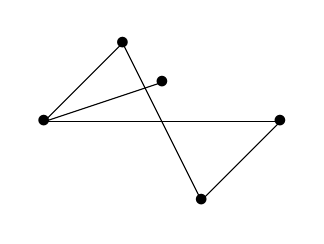
\begin{tikzpicture}
\coordinate (A) at (0,0);
\coordinate (B) at (1,1);
\coordinate (C) at (2,-1);
\coordinate (D) at (3,0);
\coordinate (E) at (1.5,0.5);

\draw (A) node {$\bullet$};
\draw (B) node {$\bullet$};
\draw (C) node {$\bullet$};
\draw (D) node {$\bullet$};
\draw (E) node {$\bullet$};
\draw (A) -- (B);
\draw (B) -- (C);
\draw (A) -- (E);
\draw (C) -- (D);
\draw (A) -- (D);
\end{tikzpicture}
\end{center}
Proposer un protocole vous permettant de visiter les tunnels afin de n'oublier aucune bibliothèque.
\item Testez votre protocole sur le réseau de tunnel de votre choix. Votre réseau devra comporter au moins $10$ bibliothèques.
\item Les bibliothèques représentent ici les pages web que le moteur de recherche souhaite référencer. À quoi correspondent alors les tunnels ?
Du point de vue de Google par exemple, cette tâche d'exploration est confiée à des robot. CHaque page web explorée de cette manière est donc envoyé à une base de données.
\end{enumerate}
\section{Classement des pages}
Bien sûr, suivant votre recherche, plusieurs pages web correspondent à ce que vous cherchez. Les moteurs de recherches ont donc la tâche de classer "par popularité" les différentes pages web afin de vous présenter les résultats les plus pertinents. D'après vous, quels seraient les critères les plus pertinents pour faire un tel classement ?

Google utilise un algorithme appelé PageRank pour noter les pages web. Faire une recherche sur cet algorithme et expliquer brièvement comment cet algorithme mesure la popularité.

\end{document}